\section{Physical Network Service Composition}
Before venturing into Virtualized Network Functions, it needs to be clarified what network functions are in general, how they are implemented and composed \textit{physically}, and what the motivations are to move towards virtualizing them. 

Networks are the backbone of any modern IT infrastructure, and with the unstoppable rise of  Cloud Computing services their importance is ever increasing. This sharp rise in relevance causes the setup and operation of previously unthinkable data centers. Providing specific functioniality in such an environment has traditionally been the task of dedicated hardware that implemented services of many different domains. These include security functions that setup firewalls, scan for viruses and detect intruders but might be applied to ``...to any data plane packet processing and control plane function...''\cite{nfv_wp}. The advantage of using ASICs (Application-specific integrated circuit) lies in the potential for optimization. When designing a device that serves a very specific purpose, the application scenario can be anticipated much better than with general-purpose hardware. This typically leads to lower power consumption, higher efficiency and better output, but drives up the purchasing cost. Additionally, the operational cost is also high, since acquiring, configuring, deploying and maintaining such middleboxes is often a tedious, manual-heavy task. 

\begin{figure}[H]
	\centering
	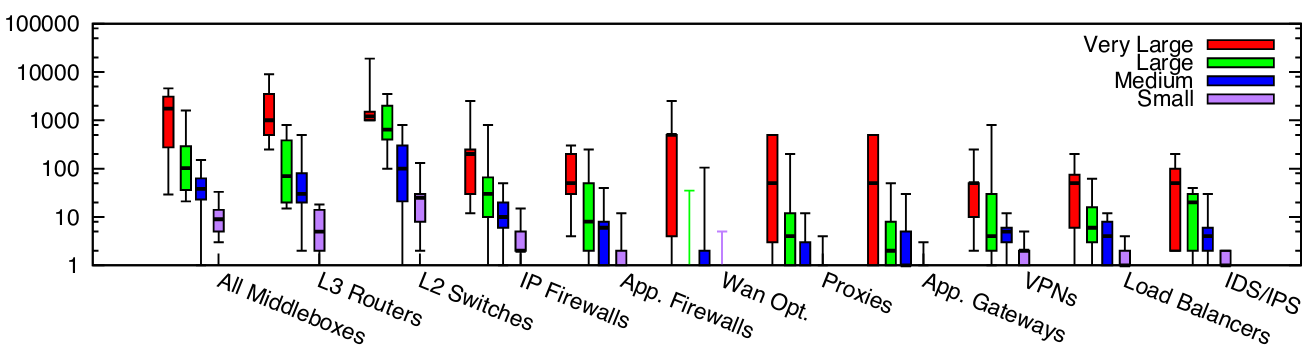
\includegraphics[width=1\linewidth]{images/middleboxesNumbers.png}
	\caption{Middlebox deployments in enterprise networks of various size (< 1k - >100k hosts). Y-axis in log scale, source \cite{sherry2016middleboxes}}
	\label{img:middleboxesNumbers}
\end{figure}

\begin{figure}[H]
	\centering
	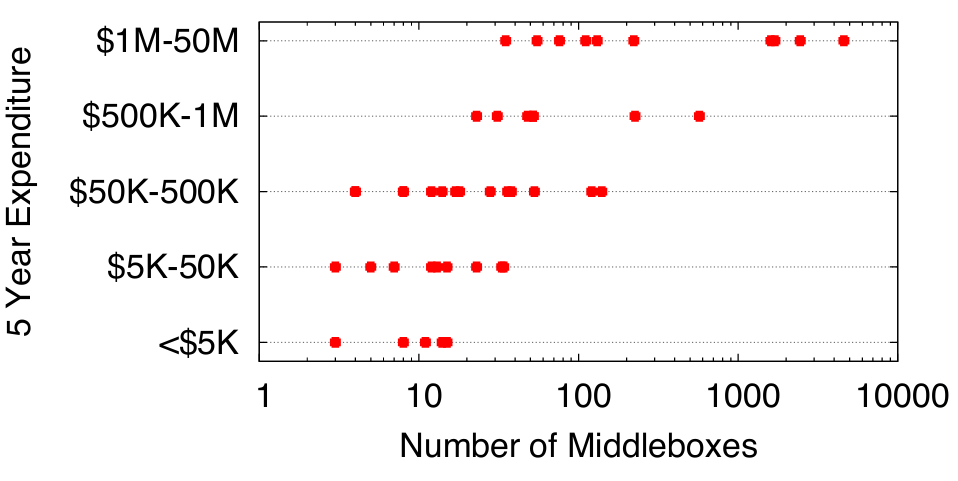
\includegraphics[width=1\linewidth]{images/middleboxesCost.png}
	\caption{Administrator-estimated spending on middlebox hardware per network \cite{sherry2016middleboxes}}
	\label{img:middleboxesCost}
\end{figure}

Figure \ref{img:middleboxesNumbers} illustrates the sheer amount of devices that are needed to guarantee the operation of enterprise networks of various size. Sherry \cite{sherry2012survey} \cite{sherry2016middleboxes} investigated their distribution among 57 educational and enterprise networks by surveying the operators for their experiences with the network appliances. Special focus was put on the quantity, their concerns, the cost and the ease of management. The results of this work give a good indication why this situation is unsustainable for future networks:  The number of these boxes is very high. To put it into perspective, the amount of these function specific devices approaches that of fundamental hardware like L3/L2 infrastructure. The associated cost of deploying such a large number of devices can be inspected in figure \ref{img:middleboxesCost} and indicates that investment cost is skyrocketing. Naturally, this might not be a problem for small companies that use a little amount of these devices. However, Cloud and Internet Service Providers rely on building, maintaining and reorganizing enormous computer networks and thus are driving forces behind alternative concepts in this domain \cite{sherry2016middleboxes} \cite{sherry2012survey}.

This will only gain importance with higher complexity and higher demand of the networks that are being built. Growing cloud data centers, implementation of 5G, further services provided in the cloud like for instance Google Stadia, a streaming service for gaming. This is a very interesting scenario since low latency and high bandwidth is of utmost importance. This project might be paving the way for more ``serious'' applications like autonomous driving. 

\section{Network Virtualization}

\subsection{Software Defined Networking}
\begin{description}
	\item [SDN] SDN: Breakup of the control and data plane, routing hardware (switches) can be organized and ()re-)configured from a distributed controller software without the need of cumbersome manual efforts.
\end{description}

\subsection{NFV and NFVI}
Network 

\begin{figure}[H]
	\centering
	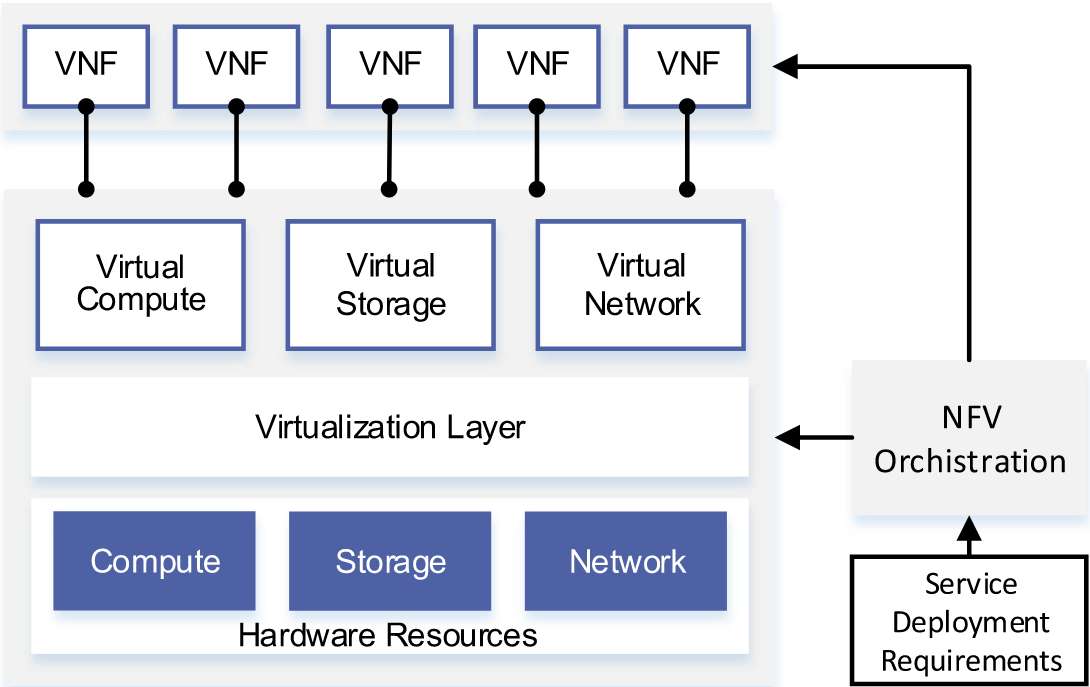
\includegraphics[width=1\linewidth]{images/nfvi.png}
	\caption{This is the caption \cite{li2015software}}
	\label{img:nfvi}
\end{figure}

\subsection{SDN and NFV}

\begin{comment}
	
In addition to the purchasing cost, the boxes have to be installed and maintained, causing administrative and operative cost. Since the nature of such devices is proprietary on a hard- and software level, training of personnel has to take vendor specific configuration into consideration. This can even influence the decision whether to invest in a specific implementation of middleboxes, since without the required expertise, the products could seriously endanger any potential profit. Scalability and fault tolerance are often enhanced by introducing additional and redundant devices into the network, adding to the operational cost. Finally, once newer functionality is released on the market, old middleboxes have no possibility of being upgraded. The only way of making use of up-to-date features is to replace the hardware in question \cite{wood2015toward} \cite{sherry2012survey} \cite{bari2015orchestrating} \cite{mekky2017network}.

Turning away from application-specific integrated circuits towards software-based solutions that can be run on general-purpose hardware is the core proposal of Network Function Virtualization. The concept of NFV has been proposed by a special interest group that is part of the European Telecommunications Standards Institute (ETSI) in a white paper in 2012 \cite{nfvWhitePaper}. Since then, the proposal has gained a lot of momentum and is taken into consideration when planing the networks of the future \cite{ordonez2017network}.

\begin{figure}[H]
	\centering
	%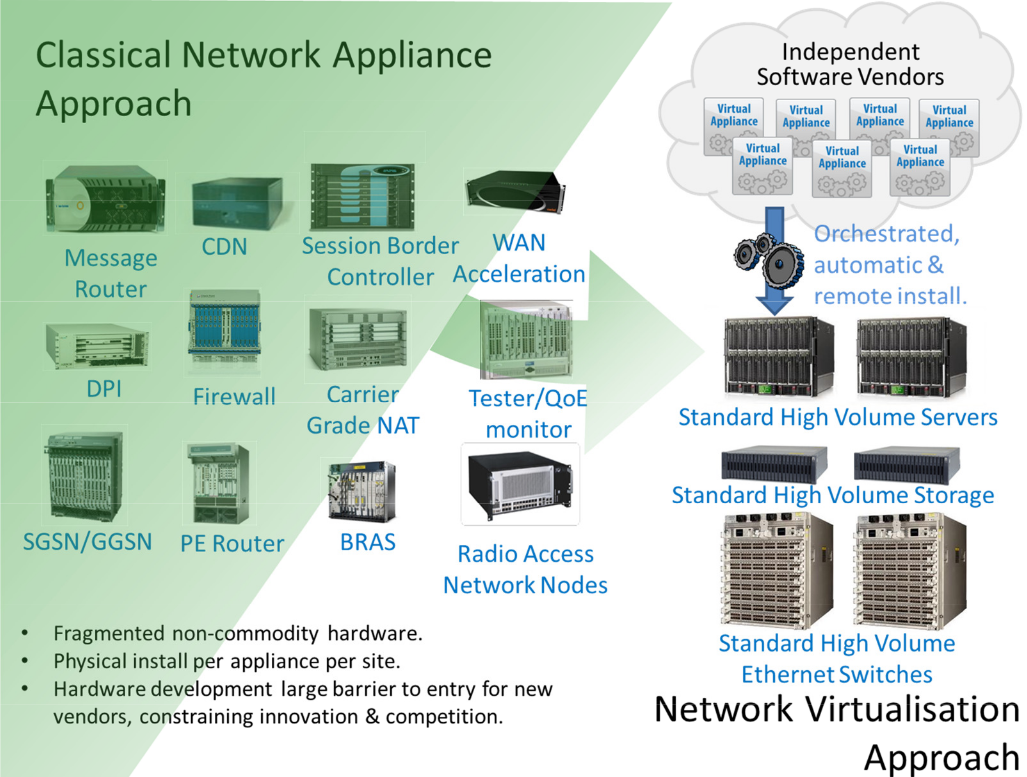
\includegraphics[width=0.85\textwidth]{images/nfv.png}
	\caption{From ASICs, to virtual appliances, source \cite{nfvWhitePaper}}
	\label{img:nfv}
\end{figure}
The core vision, as taken from the introductory white paper, is to break up the tight coupling of function and physical appliance. Figure \ref{img:nfv} shows this transition from several, tightly and vertically integrated hardware middleboxes, towards a system where the desired services are provided in virtual form by independent software vendors (top right). The underlying hardware consists of devices that can already be found in data centers, like standard high volume servers, storage and Ethernet switches. The deployment of the virtual appliances no longer requires tedious, manual and a per device setup and configuration but can rather be done in an orchestrated, automatic and remote way. The definition of such services has now also been decoupled from hardware development, favoring the emergence of a broader software ecosystem. In this environment the supply of possible network functions rises and updated or new functionality can be obtained remotely. This concept benefits highly from being used in a network environment that realizes SDN principles. The whitepaper, laying out the core principles, even includes a passage that specifies the relationship between NFV and SDN as mutually beneficial: "[...] SDN can enhance performance, simplify compatibility with existing deployments, and facilitate operation and maintenance procedures", while NFV "[...] is able to support SDN by providing the infrastructure upon which the SDN software can be run"\cite{nfvWhitePaper}. 

\end{comment}
